\section{Introducción y Objetivos}

\subsection{Introducción}
En las últimas décadas, la energía solar ha cobrado una gran relevancia, llegando a representar una parte sustancial de la generación de energía renovable a nivel mundial gracias a los avances en las tecnologías fotovoltaicas y a la creciente demanda energética \cite{IEA2023}. La expansión de la infraestructura de energía solar es un pilar fundamental para la electrificación, la transición energética global y el cumplimiento de los compromisos de cero emisiones netas para mitigar los efectos del cambio climático. Sin embargo, la generación fotovoltaica está sujeta a una alta variabilidad e intermitencia, ya que depende directamente de factores meteorológicos dinámicos como la Irradiancia Horizontal Global (GHI), la temperatura, la nubosidad y la velocidad del viento \cite{Antonanzas2016}. Por lo tanto, la estimación precisa de la productividad en plantas de energía renovable es un desafío crítico para la planificación, operación y optimización de los sistemas energéticos de la red \cite{cen2025}.

Tradicionalmente, los modelos predictivos de generación solar se han abordado mediante técnicas estadísticas y algoritmos clásicos que se entrenan de manera local utilizando los datos históricos específicos de cada planta. Este enfoque presenta dos limitaciones fundamentales. En primer lugar, dependen fuertemente de la disponibilidad de un volumen considerable de datos históricos locales, lo cual dificulta enormemente su aplicación en escenarios de puesta en marcha de nuevas instalaciones (el problema de \textit{cold-start} o arranque en frío). En segundo lugar, omiten el aprovechamiento de los patrones meteorológicos y operativos que son compartidos entre distintas plantas y regiones climáticas, los cuales poseen un alto valor para mejorar la capacidad predictiva y la generalización de los modelos.

Para superar estas barreras de disponibilidad de datos, la investigación reciente ha comenzado a integrar técnicas avanzadas de Deep Learning, donde arquitecturas como los Transformers (ej. Temporal Fusion Transformer, Informer \cite{Zhou2021} o PatchTST \cite{Nie2022}) han demostrado una capacidad superior para procesar secuencias largas y extraer dependencias temporales complejas a partir de datos meteorológicos multivariados \cite{Arslan2025}. Complementariamente, el uso de enfoques de \textit{Transfer Learning} (aprendizaje por transferencia) permite que un modelo pre-entrenado a partir de bases de datos a gran escala y de múltiples regiones transfiera características y patrones climáticos generales hacia instalaciones locales con escasez de datos \cite{Bak2025}.

El presente proyecto busca abordar el problema del \textit{cold-start} a través del desarrollo y validación de una arquitectura de "\textit{Cross-Site Learning}" (aprendizaje multi-sitio). Mediante el uso de un modelo Transformer de estado del arte, el proceso de entrenamiento se adaptará para aprender simultáneamente de múltiples series temporales de distintas plantas solares, integrando variables exógenas dinámicas (clima) y características estáticas (ubicación geográfica).

El desarrollo de este proyecto aporta valor empírico y metodológico en dos frentes principales. En primer lugar, proporciona una herramienta validada para la industria, permitiendo a los operadores estimar con mayor precisión la producción de nuevos parques solares desde sus etapas iniciales sin depender de recolecciones de datos locales prolongadas. En segundo lugar, aporta evidencia sólida sobre la eficacia de aplicar técnicas de \textit{Transfer Learning} y arquitecturas Transformer en series de tiempo energéticas, estableciendo un marco de evaluación riguroso frente a modelos tradicionales de Machine Learning (como XGBoost o LSTM) entrenados de manera estrictamente local.

\subsection{Problemática}
La transición hacia una matriz energética sostenible ha impulsado una expansión acelerada de proyectos fotovoltaicos. Tal como indica la Comisión Nacional de Energía, el 75\% de los 5.333 MW de nueva capacidad eléctrica actualmente en etapa de construcción en el país corresponde a parques solares \cite{cne2026}. Sin embargo, esta inyección masiva de energía choca con una barrera crítica para la toma de decisiones: la escasez de datos meteorológicos y operativos durante las etapas iniciales de un proyecto. Para generar proyecciones confiables y superar el problema del Cold-Start, los algoritmos predictivos tradicionales —entrenados de manera aislada para cada instalación— requieren de un mínimo de un año ininterrumpido de registros locales \cite{rodriguez2023energy}. Esto fomenta un profundo aislamiento del aprendizaje técnico, impidiendo que el conocimiento atmosférico generalizado (enfoque Multi-Sitio) se transfiera, lo que condena a los nuevos actores del mercado a operar con altos niveles de incertidumbre algorítmica desde su puesta en marcha.

Esta falta de predictibilidad a corto plazo desencadena severas ineficiencias operativas y un alto riesgo financiero a lo largo de la red. A nivel sistémico, el Coordinador Eléctrico Nacional (2025) reporta que las imprecisiones en los pronósticos de inyección renovable han introducido un error financiero del 4,62\% sobre la estimación de los costos operativos totales del Sistema Eléctrico Nacional. Más grave aún, la incapacidad de anticipar con exactitud la generación exacerba los cuellos de botella en la transmisión, derivando en niveles críticos de vertimiento de energía limpia (curtailment). Durante 2025, el vertimiento físico alcanzó los 6.084 GWh \cite{acera2025}, lo que se ha traducido en pérdidas de ingresos para las generadoras equivalentes a 562 millones de dólares acumulados en los últimos tres años \cite{ember2025}. Finalmente, en el ecosistema a menor escala, esta incertidumbre algorítmica expone directamente a los Pequeños Medios de Generación Distribuida (PMGD) a un riesgo de mermas financieras estimado en hasta 7.400 millones de dólares anuales ante la falta de certeza horaria en sus esquemas de inyección \cite{gpm2025}.

\begin{table}[htbp]
  \centering
  \resizebox{\textwidth}{!}{
  \begin{tabular}{|m{5cm}|m{3.5cm}|m{5.5cm}|}
    \hline
    \textbf{Variable / Métrica} & \textbf{Magnitud Estimada} & \textbf{Fuente de Referencia} \\
    \hline
    Capacidad solar en construcción & 75\% del total (MW) & Comisión Nacional de Energía (2026) \\
    \hline
    Error financiero sistémico & 4,62\% de costos operativos & Coordinador Eléctrico Nacional (2025) \\
    \hline
    Vertimiento físico anual & 6.084 GWh & ACERA (2025) \\
    \hline
    Pérdida por vertimiento (3 años)& 562 Millones USD & Ember (2025) \\
    \hline
  \end{tabular}
  }
  \caption{\label{tab:impacto_financiero} Resumen del impacto operativo y financiero por incertidumbre predictiva.}
\end{table}

\subsection{Cliente y/o Público objetivo}
El público objetivo y los principales beneficiarios de esta solución abarcan un espectro amplio dentro del ecosistema de generación de energía renovable. En primer lugar, la herramienta se orienta a operadores, administradores de parques solares a gran escala y coordinadores de redes eléctricas, quienes requieren sistemas predictivos robustos para minimizar la incertidumbre en la toma de decisiones, optimizando la planificación energética y reduciendo el riesgo financiero ante desvíos en el despacho durante las etapas iniciales de una planta.

En segundo lugar, esta propuesta integra a los actores del segmento de Pequeños Medios de Generación Distribuida (PMGD) y a los desarrolladores de sistemas de autoconsumo fotovoltaico a pequeña y mediana escala (comercial e industrial). Para este nicho, donde la instalación de sensórica avanzada o la recopilación de años de datos locales resulta económicamente inviable, un modelo multi-sitio pre-entrenado les permitirá acceder a proyecciones a corto plazo continuas y confiables desde su puesta en marcha, permitiendo rentabilizar sus operaciones y gestionar su inyección a la red sin la barrera de entrada que supone el modelado de datos aislado y tradicional.

\subsection{Objetivo General}
Analizar y comparar el desempeño de un modelo global de aprendizaje multi-sitio frente a modelos locales entrenados con datos históricos, en la estimación de la productividad de plantas de energía renovable, considerando su capacidad de generalización y su rendimiento en escenarios de escasez de datos e intermitencia.

\subsection{Hipótesis}
La implementación de un modelo globalmente entrenado con información proveniente de centros meteorológicamente variados, es capaz de usar información generalizada respecto de las variaciones en las condiciones atmosféricas para obtener un mejor resultado respecto de la producción de energía de una planta de producción desconocida, siendo más precisa que un modelo localmente entrenado solo con la información histórica del centro.

\subsubsection{Objetivos Específicos}
\begin{enumerate}
    \item Seleccionar y configurar una arquitectura Transformer preexistente que sea adecuada para el pronóstico de series de tiempo. Posteriormente, adaptar su proceso de entrenamiento con el fin de que el modelo sea capaz de procesar y aprender de manera simultánea a partir de múltiples series temporales provenientes de diferentes plantas solares, reemplazando así el tradicional enfoque de entrenamiento aislado.
    \item Evaluar la efectividad del modelo global pre-entrenado durante la puesta en marcha de una nueva planta renovable que cuente con una escasa cantidad de datos con respecto a modelos tradicionales (como XGBoost o LSTM) entrenados de manera estrictamente local.
    \item Integrar datos multimodales para dotar al modelo de la capacidad de procesar diversas fuentes de información, integrando de manera conjunta tanto variables exógenas dinámicas, que representan las condiciones meteorológicas, como características estáticas referentes a la ubicación espacial y geográfica de cada estación.
\end{enumerate}

\subsection{Alcance del Proyecto}
Con el propósito de analizar y comparar el desempeño predictivo de modelos globales frente a modelos locales, el alcance de este proyecto se focaliza en el dominio de la producción de energía solar mediante el estudio de un conjunto consolidado de instalaciones agrupadas bajo un criterio de Macrozona. Esta estrategia de agrupación responde a la necesidad de estabilizar las características climáticas compartidas y escalar el aprendizaje cruzado entre plantas. Esta configuración experimental permite integrar series de tiempo de producción y variables meteorológicas de alta fidelidad para evaluar la capacidad de generalización y la respuesta del modelo ante la escasez de datos. Técnicamente, el trabajo se concentra en la parametrización, el entrenamiento multi-sitio y la validación de arquitecturas de estado del arte (TFT, Informer, N-HiTS), empleando modelos XGBoost y LSTM como líneas base comparativas. Finalmente, para mantener el foco en la evaluación del rendimiento del modelado, se excluyen explícitamente el desarrollo de nuevas estrategias o metodologías desde cero, el despliegue en entornos de producción (MLOps), la integración con sistemas SCADA y cualquier análisis de viabilidad financiera o rentabilidad operativa sobre los activos estudiados. De manera que el proyecto se compone de la recopilación y preprocesado de datos, la configuración de la estrategia de orquestación para el testeo, el entrenamiento de los modelos base, la ejecución y posterior comparación entre el modelo globalmente entrenado y las baseline en situaciones de ``Cold-Start''. Todo circunscrito por un repositorio con los pipelines de datos, entrenamiento y posterior testeo.

\begin{figure}[htbp]
  \centering
  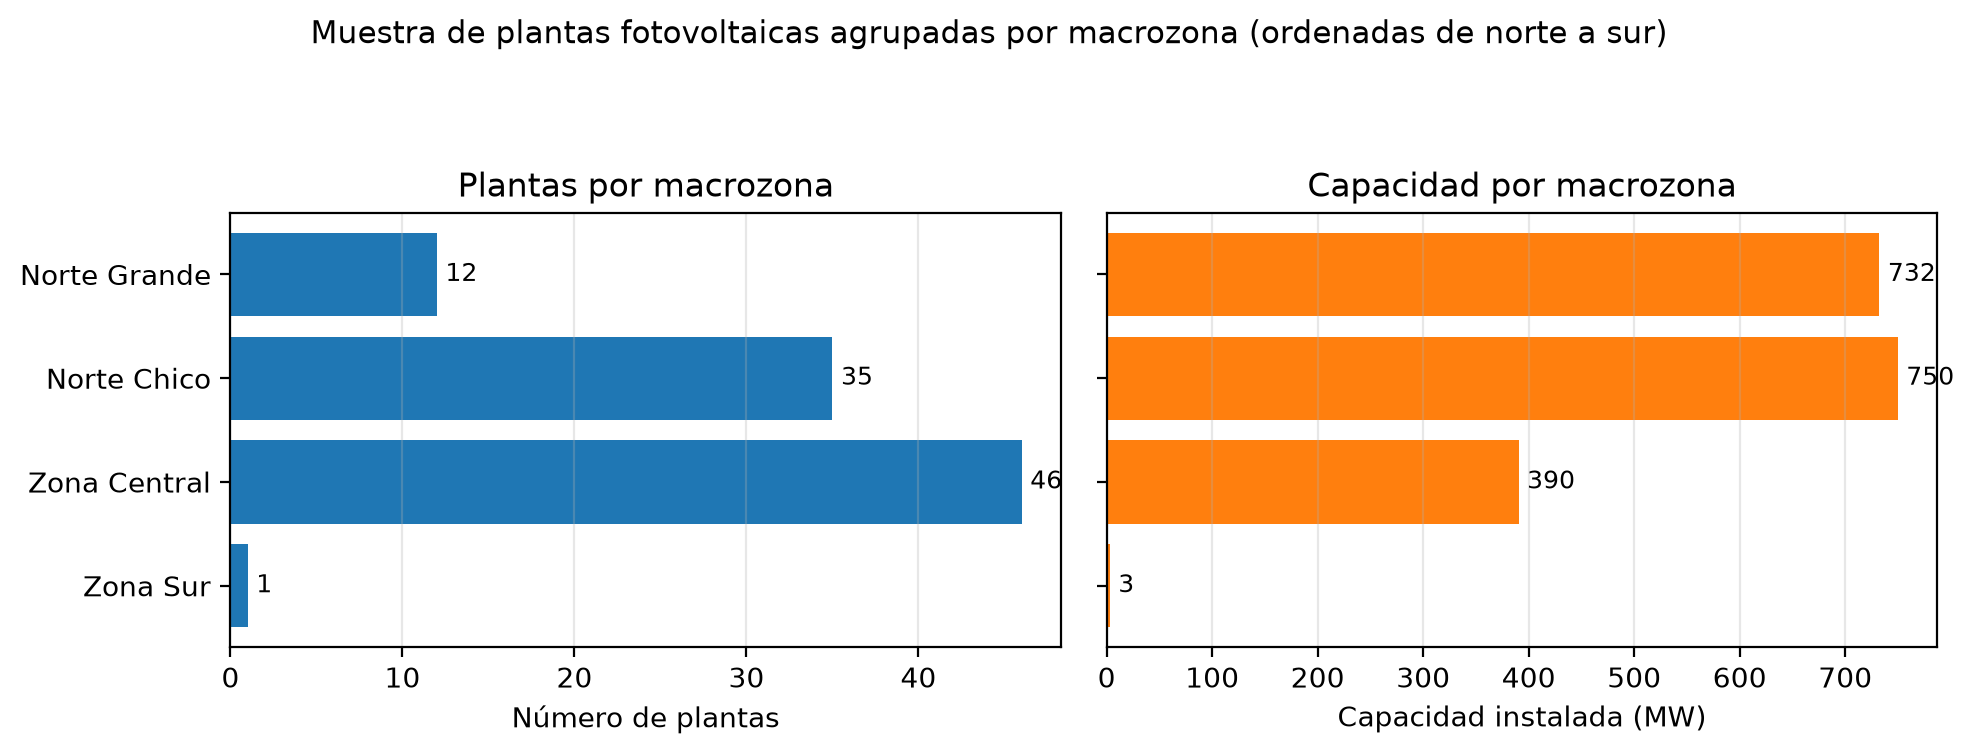
\includegraphics[width=\textwidth]{figuras/fig_mapa_muestra.png}
  \caption{\label{fig:mapa_alcance} Distribución de las plantas fotovoltaicas de la muestra por macrozona (94 instalaciones; 1.876 MW de capacidad agregada).}
\end{figure}

\subsection{Carta de Compromiso}
Dada la naturaleza de la presente investigación, el desarrollo del modelo no se encuentra aunado a la intervención o patrocinio exclusivo de una entidad privada específica para su ejecución técnica. El acceso a los activos de datos necesarios para el cumplimiento de los objetivos planteados ha sido gestionado bajo protocolos internos, lo que garantiza la viabilidad y autonomía del estudio en sus etapas de entrenamiento y validación. No obstante, se mantiene la disposición para formalizar vínculos de colaboración técnica con organismos del sector en fases posteriores, con el fin de robustecer la transferencia tecnológica de los resultados obtenidos.

\newpage

\subsection{Planificación del Trabajo (Carta Gantt)}
Para cumplir con los objetivos trazados de manera sistemática, se ha definido una carta Gantt de seis semanas de duración orientada a la ejecución técnica, evaluación del \textit{Cold-Start} y consolidación de resultados (ver Figura \ref{fig:gantt_planificacion}).

\begin{figure}[htbp]
  \centering
  \begin{ganttchart}[
      hgrid, vgrid,
      x unit=1.5cm, y unit chart=0.62cm, y unit title=0.7cm,
      title/.append style={fill=ucmblue!15},
      title label font=\small\bfseries,
      bar/.append style={rounded corners=1pt},
      bar label font=\small,
      bar height=0.6
    ]{1}{6}
    \gantttitle{Semanas de ejecución}{6} \\
    \gantttitlelist{1,...,6}{1} \\
    \ganttbar[bar/.append style={fill=obj3}]{Procesamiento de datos multimodales}{1}{2} \\
    \ganttbar[bar/.append style={fill=obj2}]{Entrenamiento algoritmos clásicos}{2}{3} \\
    \ganttbar[bar/.append style={fill=obj1}]{Parametrización arquitectura Transformer}{2}{3} \\
    \ganttbar[bar/.append style={fill=obj1}]{Entrenamiento simultáneo Cross-Site}{3}{4} \\
    \ganttbar[bar/.append style={fill=obj2}]{Simulación Cold-Start}{4}{5} \\
    \ganttbar[bar/.append style={fill=obj2}]{Benchmark comparativo y métricas}{5}{6} \\
    \ganttbar[bar/.append style={fill=general}]{Redacción y entrega final}{1}{6}
  \end{ganttchart}
  \vspace{4pt}

  {\small
    \textcolor{obj1}{$\blacksquare$}~Obj.~1: Arq.~Transformer \quad
    \textcolor{obj2}{$\blacksquare$}~Obj.~2: Eval.~Cold-Start \quad
    \textcolor{obj3}{$\blacksquare$}~Obj.~3: Datos multimodales \quad
    \textcolor{general}{$\blacksquare$}~Tareas transversales}
  \caption{\label{fig:gantt_planificacion} Planificación estructurada en 6 semanas, categorizada según los Objetivos Específicos del proyecto.}
\end{figure}